%!TEX root = ../../Compte-rendu.tex


\begin{figure}[H]
	\begin{center}
		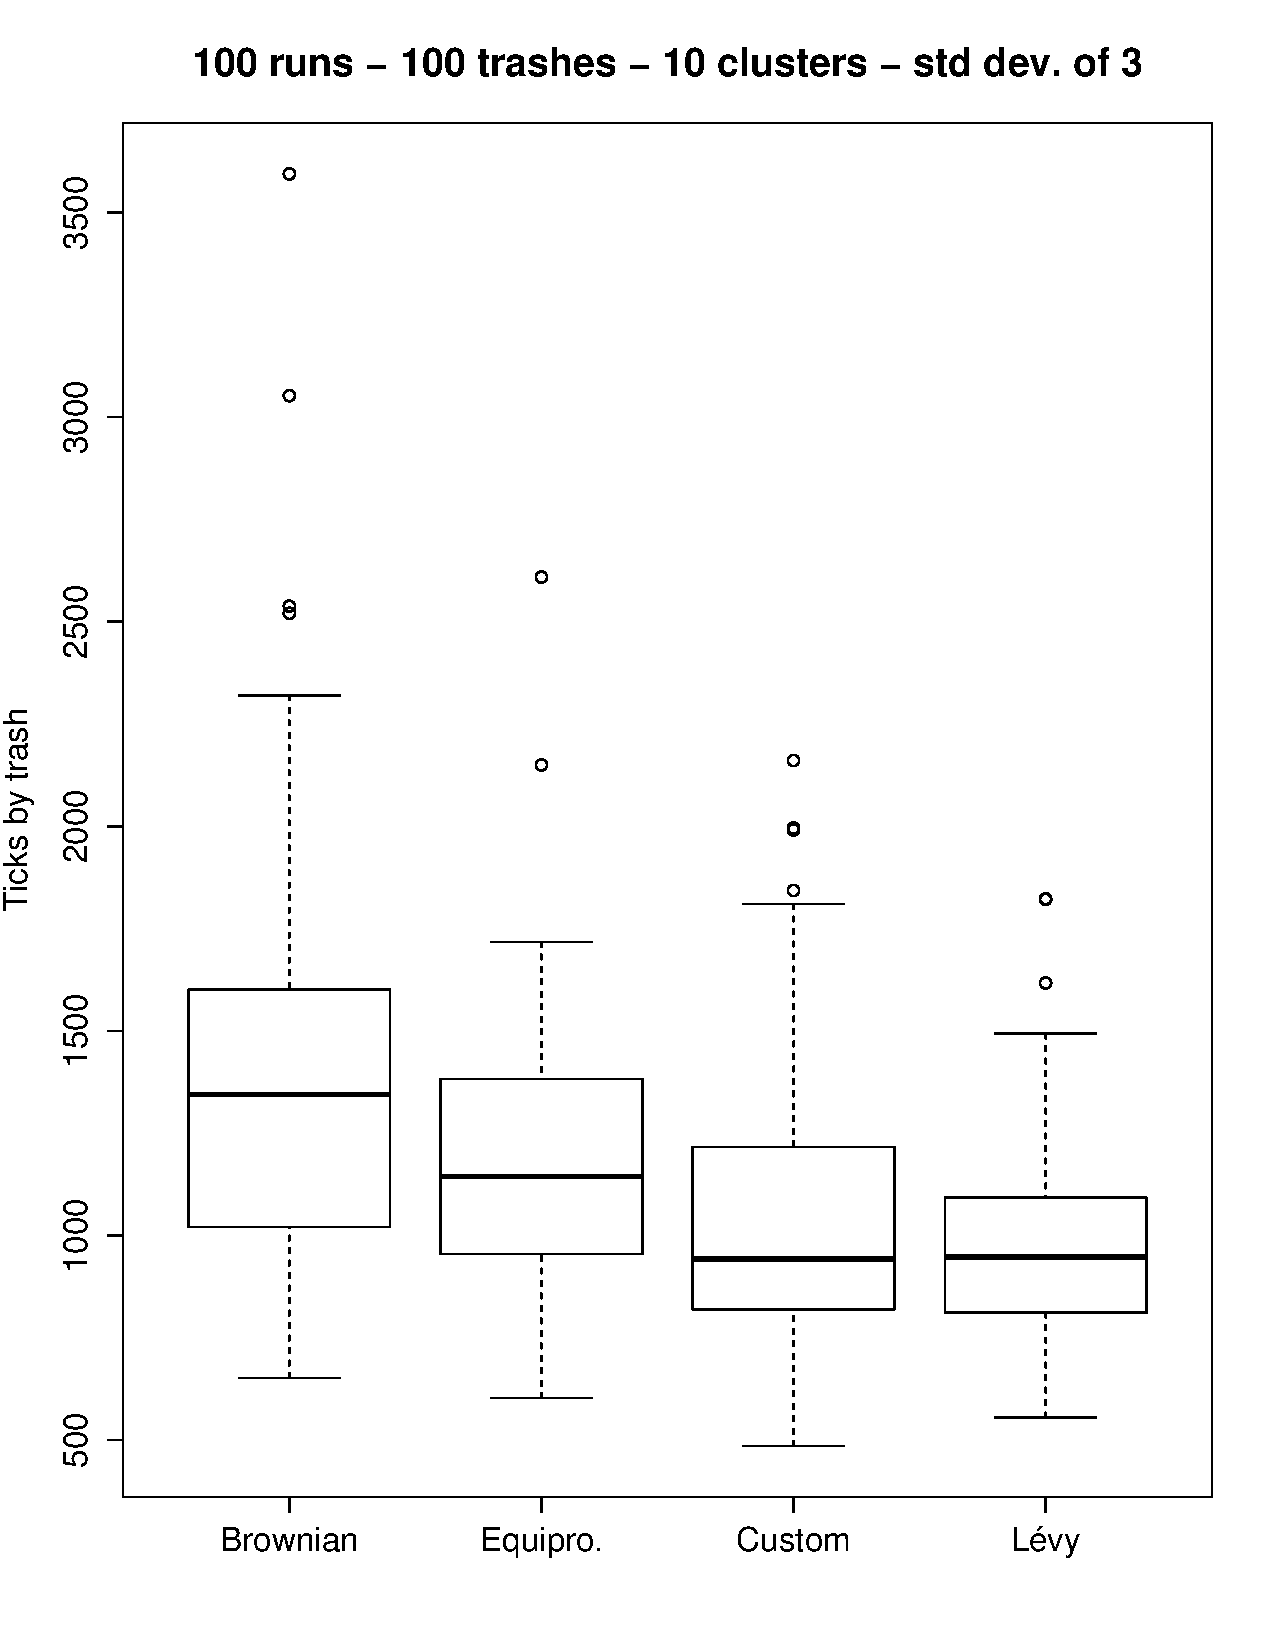
\includegraphics[height=10cm]{diagrams/100Tr10Clts_all.pdf}
		\caption{Résultat des mesures pour 100 débris distribué en 10 clusters (écart-type 3)}
		\label{fig:100Trashes_10Clusters}
	\end{center}
\end{figure}

Nous avons pour les différentes stratégies les statistiques suivantes :

\begin{figure}[H]
	\begin{center}
		\begin{tabular}{| c || c | c | c | c | }
			\hline
			&Brown.&Equi.&Custom&Lévy \\
			\hline
			\hline
			md&1344&1144&942&947\\
			mean&1388&1187&1053&984\\
			min & 652 & 602 & 485 & 555 \\
			max & 3595 & 2609 & 2161 & 1823 \\
			sd&491&318&344&256\\
			p-val&$\ll 5\%$&$\ll 5\%$&$\ll 5\%$&$\ll 5\%$\\
			\hline
		\end{tabular}
		\caption{Statistiques pour 100 débris distribué en 10 clusters (écart-type 3)}
	\end{center}
\end{figure}


Nous pouvons constater que la stratégie Custom a une médiane très
légèrement meilleure à la stratégie Lévy, néanmoins cette première
est moins fiable, c'est à dire qu'elle a plus de chance de produire
des résultats bien moins bons que le Lévy.

Nous pouvons aussi voir que la stratégie Custom perd en fiabilité
alors que la stratégie Equiprobable, elle, en gagne.